% Modified by Muhammed Yavuzhan CANLI, 25 July 2025

\documentclass[12pt,a4paper]{report}
\usepackage[utf8]{inputenc}
\usepackage[T1]{fontenc}

\usepackage{enumitem}
\usepackage[utf8]{inputenc}
\usepackage[T1]{fontenc}
\usepackage{Bath-CS-Dissertation}
\usepackage{lmodern}         % scalable font fix
\usepackage{float}          

\title{\bf Enhancing Customer Engagement in Physical Casino Environments through Machine Learning-Powered Segmentation and Prediction}
\author{Muhammed Yavuzhan CANLI}
\date{MSc in Computer Science\\
      The University of Bath\\
      Academic Year: 2024--2025\\
      \vspace*{5cm}
      The University of Bath - Ethical Approval: 10351-12382}

\setcounter{secnumdepth}{3}
\setcounter{tocdepth}{3}


%%%%%%%%%%%%%%%%%%%%%%%%%%%%%%%%%%%%%%%%%%%%%%%%%%%%%%%%%%%%%%%%%%%%%%%%%%%%%%%%
%%%%%%%%%%%%%%%%%%%%%%%%%%%%%%%%%%%%%%%%%%%%%%%%%%%%%%%%%%%%%%%%%%%%%%%%%%%%%%%%
%%%%%%%%%%%%%%%%%%%%%%%%%%%%%%%%%%%%%%%%%%%%%%%%%%%%%%%%%%%%%%%%%%%%%%%%%%%%%%%%
\usepackage{amsmath}
\usepackage{amssymb}
\usepackage{url}  

\begin{document}
\sloppy
\tableofcontents


\hypersetup{pageanchor=false}

% Set this to the language you want to use in your code listings (if any)
\lstset{language=Java,breaklines,breakatwhitespace,basicstyle=\small}

\setcounter{page}{0}
\pagenumbering{roman}

\maketitle
\newpage

% Set this to the number of years consultation prohibition, or 0 if no limit
\consultation{0}
\newpage

\declaration{Enhancing Customer Engagement in Physical Casino Environments through Machine Learning-Powered Segmentation and Prediction}{Muhammed Yavuzhan CANLI}

\newpage

\hypersetup{pageanchor=true}

\abstract
The development of artificial intelligence (AI) has created new possibilities for improving decision-making processes in physical casino settings.  Traditional casinos encounter structural and technological obstacles in the integration of data sources, including slot logs, ticket-in ticket-out (TITO) systems, and customer relationship management (CRM) databases, unlike online platforms.  This dissertation examines the creation of a machine learning framework designed to enhance promotional decision-making within a physical casino environment.

 The proposed system employs a hybrid data architecture and applies unsupervised learning through K-Means clustering to classify customers based on behavioural and demographic indicators.  A Random Forest classifier is employed to predict engagement levels with targeted promotions, and its performance is evaluated against alternative algorithms (SVM, Decision Tree, and Logistic Regression) to ensure robustness.

  The system is organised with a PostgreSQL database backend, Python-based AI modules, and a Docker deployment environment.  Data is anonymised, ethically sourced, and processed in accordance with the University of Bath's ethics guidelines (Approval Ref: 10351-12382) \citep{bathEthics}.

 This study presents a modular, reproducible, and scalable methodology for customer analytics within the casino sector.  The system enables casino IT personnel to make informed, real-time decisions regarding promotion targeting, thus enhancing operational efficiency and customer engagement while maintaining data privacy.
\newpage

\tableofcontents
\newpage

\listoffigures
\newpage

\listoftables
\newpage

%%%%%%%%%%%%%%%%%%%%%%%%%%%%%%%%%%%%%%%%%%%%%%%%%%%%%%%%%%%%%%%%%%%%%%%%%%%%%%%%
%%%%%%%%%%%%%%%%%%%%%%%%%%%%%%%%%%%%%%%%%%%%%%%%%%%%%%%%%%%%%%%%%%%%%%%%%%%%%%%%
\chapter*{Acknowledgements}

Add any acknowledgements here.

\newpage
\setcounter{page}{1}
\pagenumbering{arabic}

%%%%%%%%%%%%%%%%%%%%%%%%%%%%%%%%%%%%%%%%%%%%%%%%%%%%%%%%%%%%%%%%%%%%%%%%%%%%%%%%
%%%%%%%%%%%%%%%%%%%%%%%%%%%%%%%%%%%%%%%%%%%%%%%%%%%%%%%%%%%%%%%%%%%%%%%%%%%%%%%%
\chapter{Introduction and Background}

The rise of artificial intelligence (AI) in recent years has profoundly reshaped industries that rely on data-driven decision-making. In particular, the casino industry historically reliant on intuition, human observation, and loyalty-based marketing now stands at a transformative intersection. Unlike online gambling platforms that are inherently digital, physical casinos face more complex challenges when it comes to integrating operational, behavioural, and demographic data sources for intelligent decision-making.

This dissertation addresses the pressing need for a structured, ethical, and technically robust framework that enhances customer engagement in physical casinos. Through the development of an AI-powered decision support system, this research combines customer segmentation with behavioural analytics to support dynamic promotional strategies.



%%%%%%%%%%%%%%%%%%%%%%%%%%%%%%%%%%%%%%%%%%%%%%%%%%%%%%%%%%%%%%%%%%%%%%%%%%%%%
\section{Background}

Customer retention and personal engagement are key success factors in the gambling industry. This is especially true in competitive markets where both physical and online casinos compete for player attention. Online platforms can track user behaviour in detail, but physical casinos often lack integrated systems that connect slot machine logs, ticket-in and ticket-out (TITO) data, CRM systems, and behavioural metrics. As a result, these casinos miss opportunities to personalise promotions and engagement based on customer value and risk levels.

Recent developments in machine learning—such as clustering and classification algorithms—enable new ways to extract insights from customer data. However, applying these methods in land-based casinos is more complex due to operational limitations and strict regulatory requirements. Therefore, the effective and responsible use of AI in this setting requires a combined technical and ethical framework.


%-------------------------------------------------------------------------------
\subsection{The Role of Personalisation in Casino Environments}

Personalisation is fundamental to retention and engagement with customers strategies in diverse sectors, including the casino industry.  In physical casino environments, customising the player experience serves as a competitive advantage and significantly contributes to enhanced dwell time, session value, and overall player satisfaction.

 Traditional casinos frequently depend on visible behavioural indicators and manual customer relationship management strategies to provide a personalised experience.  However, these methods exhibit constraints in both scope and scale.  Digital platforms demonstrate that data-driven personalisation, using customer profiles, interaction history, and predictive modelling, can markedly improve relevance and responsiveness in real time.


 In casinos that are physical, the integration of behavioural data from slot machines, loyalty systems, and ticket-in/ticket-out (TITO) logs enables operators to more effectively segment players and customise offers that align with individual preferences and risk profiles.  A frequent player exhibiting stable betting patterns may receive loyalty bonuses, whereas a high spending yet unpredictable player could gain more from targeted retention campaigns.

 With the increasing availability of data in casino operations, the potential for applying machine learning to enhance personalisation expands.  This project leverages the identified opportunity to enhance targeted promotional strategies via automated segmentation and response prediction mechanisms.


%-------------------------------------------------------------------------------
\subsection{The Gap Between Online and Physical Casino Analytics}

Online casinos leverage fully integrated digital frameworks that provide real-time monitoring of user activities, preferences, and transaction records.  These platforms frequently utilise sophisticated analytics and recommendation systems driven by machine learning to customise user experiences, enhance promotions, and identify undesirable activity on a large scale.  Each click, spin, and session is carefully recorded, fostering a robust framework for data-informed decision-making.

 Conversely, real casinos often function with disjointed systems.  Slot machine logs, TITO (Ticket-In Ticket-Out) records, loyalty program data, and demographic information are frequently isolated or manually aggregated.  This absence of integration diminishes the casino's capacity to develop a holistic profile of player conduct.  Consequently, promotional techniques in physical retail environments may be postponed, generic, or reliant on obsolete heuristics.

 Addressing this gap requires both technological advancement and legislative comprehensive.  Physical casinos must navigate stricter compliance requirements, restricted digital existence, and immediate limits in client engagements.  To provide equivalent analytical capabilities to their online counterparts, these environments need to implement anonymised data pipelines, centralised databases, and AI systems capable of functioning among operational complexity and ethical supervision.

%-------------------------------------------------------------------------------
\subsection{The Rise of AI-Based Promotional Systems}

%-------------------------------------------------------------------------------

\subsection{Key Concepts}
\subsubsection{Demographics as Predictors of Player Behaviour}

The analysis of age, gender, and nationality plays a crucial role in interpreting gaming behaviours, such as session frequency, risk tolerance, and betting preferences. This study adopts a regionally focused demographic design—primarily players from Bulgaria, Turkey, Greece, and other neighbouring countries—to isolate socio-cultural gaming patterns. These features were algorithmically embedded into anonymised records and integrated into behavioural pipelines, enabling segmentation and promotional targeting models to reflect demographic sensitivities.



\subsubsection{K-Means Clustering}

K-Means clustering is an unsupervised machine learning method employed to segment data into a specified number of groups according to feature similarity.  This method facilitates the identification of unique behavioural profiles—namely Casual, Regular, and High-Value players—by categorising individuals based on their gaming activity patterns, demographic attributes, and engagement metrics.

 The system progressively allocates players to the closest cluster centroid by reducing within-cluster variation.  Upon achieving convergence, each player is linked to a section that represents their comprehensive behavioural and demographic profile.  This enables customised marketing campaigns, as clusters may be analysed and categorised based on corporate goals.

 This study employed K-Means clustering on a dataset enriched with variables including average bet amount, session frequency, loss-chasing behaviour, session volatility, and recent engagement trends.  Furthermore, demographic characteristics—such as age group, gender, and nationality—were algorithmically integrated into the feature space to improve cluster differentiation and facilitate socio-cultural segmentation.

 Incorporating demographic characteristics allows the segmentation engine to uncover international gaming behaviours, age-related risk tolerances, and gender-specific promotional reactions.  Preliminary exploratory clustering indicated that younger age groups likely to engage in play more frequently but with lower betting amounts, whereas elderly players may participate less often but with bigger risks.  Additionally, participants from particular national origins demonstrated similar temporal patterns or preferred specific game kinds.

 These insights provide operational value for real-time CRM targeting and establish a basis for more profound study in subsequent rounds of this project, where cross-segment behaviours and promotion response rates will be evaluated.

The K-Means algorithm aims to minimise the intra-cluster variance by assigning each data point to the nearest cluster centroid. This is formalised by the following cost function:

\begin{equation}
\underset{S}{\arg\min} \sum_{i=1}^{k} \sum_{x \in S_i} \| x - \mu_i \|^2
\end{equation}

\begin{itemize}
    \item \( S = \{S_1, S_2, ..., S_k\} \): set of clusters.
    \item \( x \in S_i \): data point \(x\) assigned to cluster \(S_i\).
    \item \( \mu_i \): centroid of cluster \(S_i\).
    \item \(sum_{i=1}^{k}\): The total of these accounts throughout all clusters (e.g., casual, regular, high-value).
    \item arg min: Identify the cluster that minimises this total value. 
\end{itemize}

This function computes the total squared distance between each point and its assigned cluster centre across all \(k\) clusters. The goal is to find a cluster assignment \(S\) that minimises this total distance.

\vspace{0.5em}
\textbf{Example Application:} Suppose we have three customers with average bet values \(\{20, 22, 95\}\). If \(k = 2\) clusters, K-Means may assign \{20, 22\} to one cluster with centroid \(\mu_1 = 21\) and \{95\} to another with centroid \(\mu_2 = 95\), thereby minimising the squared differences:
\[
(20 - 21)^2 + (22 - 21)^2 + (95 - 95)^2 = 1 + 1 + 0 = 2
\]

This objective ensures similar players are grouped, enabling behavioural segmentation and personalised targeting.

In summary, K-Means performs the following:
\textit{``I categorise the players into clusters. However, these clusters must be arranged so that each player is positioned as near as possible to the centre of their group. In this manner, similar players are grouped together.''}


\subsubsection{Random Forest Classifier}

Random Forest is a popular ensemble learning technique that generates multiple decision trees during training and produces the class according to the majority decision across all trees \citet{randomforest}.  In contrast to a single decision tree, which is at risk of overfitting, Random Forest improves generalisation by averaging the predictions of multiple trees trained on diverse bootstrap data sets and groups of features.

Mathematically, given a training dataset \( D = \{(x_1, y_1), \dots, (x_n, y_n)\} \), Random Forest constructs \( T \) decision trees \( \{h_1(x), h_2(x), \dots, h_T(x)\} \), where each \( h_t \) is trained on a random subset of \( D \). For classification, the ensemble output \( H(x) \) is defined as:

\[
H(x) = \text{mode}\left( h_1(x), h_2(x), \dots, h_T(x) \right)
\]

This election method fixes predictions and facilitates probabilistic outputs. For instance:  
\textit{``Player A has a 74\% probability of accepting the promotion based on their loss pattern, session duration, and customer segment.''}

This research employs Random Forest to predict the possibility of promotional approval based on behavioural features, including:

\begin{itemize}
    \item Average session loss
    \item Duration and frequency of play
    \item Segment membership (e.g., Casual, High-Value, Regular)
    \item Engagement trend (e.g., bet increase/decrease)
    \item Demographic inputs (age group, gender, nationality)
\end{itemize}

\paragraph{Illustrative Example:}To illustrate how Random Forest works in the context of casino promotions, consider the following scenario:

\begin{quote}
    A casino is evaluating the potential implementation of a promotion for Player-A.  Several decision trees are developed applying historical data, with each tree employing different player subsets and features including age, gender, session duration, and loss amount.
    
    \begin{itemize}
        \item Tree-1 predicts: \texttt{Yes}
        \item Tree-2 predicts: \texttt{Yes}
        \item Tree-3 predicts: \texttt{No}
        \item Tree-4 predicts: \texttt{Yes}
        \item Tree-5 predicts: \texttt{Yes}
    \end{itemize}
    
    Out of 5 trees, 4 suggest offering a promotion. Therefore, the final output of the Random Forest is: \textbf{Yes, with 80\% confidence}.
\end{quote}

This simple majority voting method allows Random Forest to generate consistent and accurate projections, even when individual decision trees may be poor or overfitted.  The probabilistic output (e.g., 80\% likelihood) allows CRM systems to rank or filter participants according to probability, therefore prioritising marketing initiatives.

 A major advantage of Random Forest is its inherent capability of evaluating feature importance, measuring the contribution of each input variable to overall prediction effectiveness.   This enables transparency and clarity, which are particularly crucial in regulated environments such as casinos, where understanding the impact of demographic elements is essential for responsible and ethical promotional decision-making.


\subsubsection{ML vs Rule-Based Systems}

Traditional rule-based systems in casinos function through established "if-then" logic, where particular thresholds activate promotional or operational reactions—such as granting a bonus following a loss of €1000 or delivering notifications dependent on the time of day.  These systems show transparency and allow for auditing; nevertheless, they lack adaptation to dynamic behavioural patterns and are not capable of detecting underlying behavioural trends.

 On the contrary, machine learning (ML) methodologies—such as K-Means clustering and Random Forest classification—facilitate pattern recognition through the analysis of historical data.  These models clarify non-linear and complicated interactions, such as recognising that players of a particular nationality, within a defined age brackets, and exhibiting rapid recovery from losses may exhibit enhanced responsiveness to specific rewards.

 Machine learning systems provide probabilistic predictions rather than binary rule outputs, assigning probability scores to client behaviours.  This facilitates complex decision-making, for instance, "Player A has a 74\% probability of accepting a cashback promotion," so benefiting in prioritisation and risk-adjusted intervention strategies.  However, machine learning models require a resilient data infrastructure, validation methodologies, and ethical protections, especially in regulated sectors such as gaming.

 This study employs a rule-based methodology as a comparative benchmark, while the machine learning pipeline is engineered to provide scalable, real-time, and ethically acceptable promotion methods.  The two paradigms are utilised simultaneously to combine interpretability with predictive efficiency.

\vspace{0.2cm}
\textbf{Example Paradigms}:
\begin{itemize}
    \item \textbf{Rule-Based:} ``If a customer’s net loss exceeds €1000, then offer a standard promotion.''
    \item \textbf{ML-Based:} ``There is a 74\% probability that this customer will respond positively to a cashback offer, based on session length, recent losses, and demographic profile.''
\end{itemize}

%-------------------------------------------------------------------------------

\section{Problem Statement}

Problem Statement

 Despite major investments in digital infrastructure, many physical casinos continue in utilising static and intuition-based promotional strategies.  These approaches are generally predefined and lack the adaptability necessary to detect real-time variations in player activity.  Consequently, chances to improve player engagement, retention, and lifetime value are often ignored.

 In a progressively competitive landscape—where both digital and physical establishments vie for attention—comprehending player profiles has become essential.  Critical behavioural indicators, like session duration, bet size changes, recent loss patterns, and play frequency, provide significant information.  In the absence of precise measurement and evaluation of these features, traditional casinos find it challenging to customise promotional offers or identify high-value and at-risk customers.

 The lack of dynamic segmentation, real-time behavioural scoring, and predictive modelling decreases marketing efficiency and enhances the possibility of violating responsible gambling regulations.  Lack of ability to identify loss-chasing behaviours or player exhaustion may result in reputational harm or regulatory penalties.

 This study presents a modular and scalable AI-driven architecture that integrates multi-source data, including slot logs, TITO, and CRM records, within a GDPR-compliant PostgreSQL framework to overcome these limitations.  The method uses unsupervised clustering and supervised classification to produce promotional decisions tailored to specific segments.  This approach is intended to function within the operational limitations of physical casinos while supporting ethical, real-time decision-making via comprehensible machine learning techniques.


\section{Overview and Scope}

This dissertation develops, implements, and evaluates a complete AI-driven pipeline designed to enhance promotional decision-making within land-based casino environments. The proposed system combines behavioural data with synthetic demographic variables to support ethical and personalised customer engagement. The architecture is modular, scalable, and designed to be technically feasible within real-world casino operations.

The solution consists of two core components:

\begin{itemize}
    \item \textbf{Hybrid Data Integration Layer:} Behavioural data—including slot machine logs and TITO transactions—are consolidated with synthetically generated demographic attributes (age, gender, nationality) into a PostgreSQL database. All records are anonymised to ensure full compliance with GDPR regulations. The database schema was designed and implemented by the author, supporting structured, queryable datasets for downstream machine learning processes.
    
    \item \textbf{AI-Based Decision Engine:} A two-stage machine learning strategy is adopted. First, unsupervised K-Means clustering segments players into behavioural groups (e.g., Casual, Regular, High-Value). Then, a Random Forest classifier predicts individual promotional responsiveness, using behavioural features such as average loss, session duration, and volatility indicators. Additional mechanisms—such as loss-chasing detection and temporal engagement labelling—are integrated to support responsible gambling.
\end{itemize}

The pipeline is fully automated using Python modules and is deployable through a Docker-based environment. Although the system does not directly interface with a live CRM, it provides segment labels and promotion decision flags in export-ready formats compatible with casino marketing operations.

Overall, the system is designed to support ethical, transparent, and data-driven promotional strategies that respect both player privacy and operational practicality.

\begin{figure}[H]
\centering
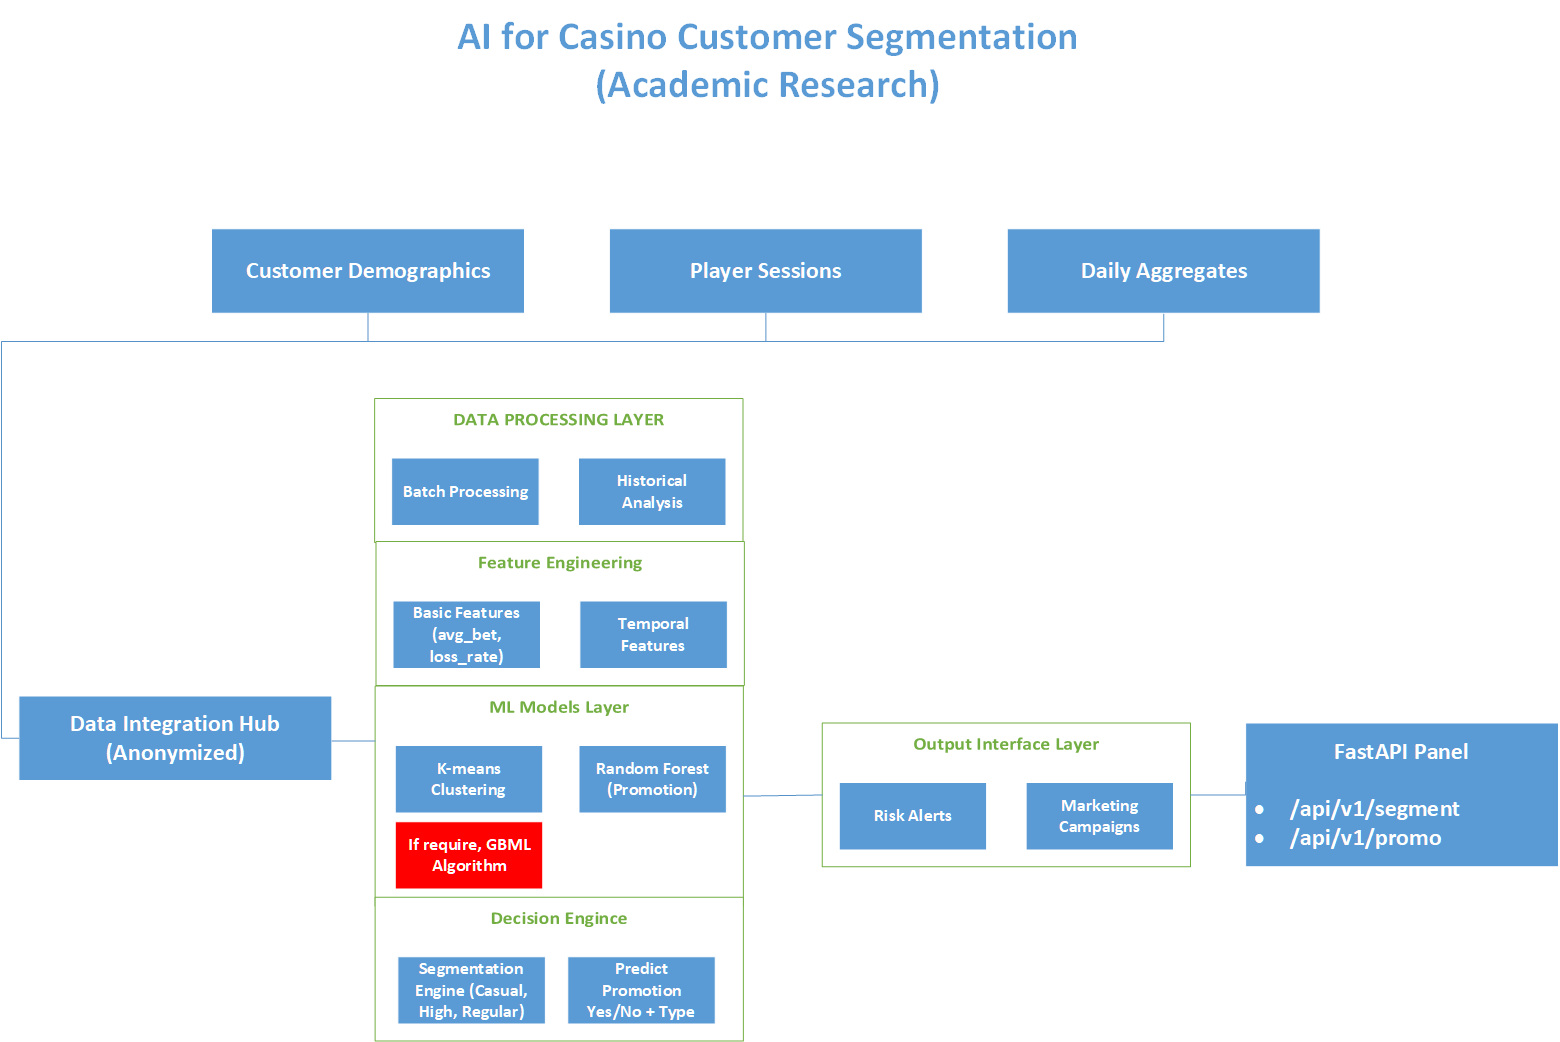
\includegraphics[width=0.9\textwidth]{figures/project_overview_diagram.png}
\caption{Project Overview: Modular Architecture Integrating Anonymised Data, Feature Engineering, and ML-Driven Promotional Decision-Making}
\label{fig:overview and scope}
\end{figure}

Illustrates the overall AI pipeline and data integration strategy. It highlights how anonymised inputs from slot logs, demographic synthesis, and behavioural records flow through the processing layer and machine learning modules to support intelligent promotional decisions and segment-aware CRM interventions.

\subsection{System Architecture and Project Pipeline Overview}
The suggested system's design is organised into a modular pipeline that integrates data ingestion, preprocessing, unsupervised clustering, supervised classification, and promotion flagging. Each module was created utilising Python and follows to a reproducible, testable approach incorporated within a Dockerized environment.

\begin{itemize}
    \item \textbf{Data Ingestion Layer:} Involved the cleaning, validation, and importation of raw behavioural logs from slot machines and TITO transactions into a PostgreSQL database. Synthetic demographic variables—age group, gender, and nationality—were algorithmically generated using the synthetic data toolkit to emulate CRM-like completeness while maintaining GDPR compliance \citep{faker2025}.

    \item \textbf{Feature Engineering:} Custom Python modules were utilised to extract behavioural metrics, including average bet, session duration volatility, loss-chasing indicators, and recent engagement trends. The features were organised within a specific \texttt{customer\_features} table, serving as the foundation for both clustering and classification processes.

    \item \textbf{Unsupervised Segmentation (K-Means):} Customers were grouped into segments (e.g., Casual, Regular, High-Value) using K-Means clustering. Segment assignments were stored in a separate table and served as contextual inputs for subsequent analysis.

    \item \textbf{Supervised Classification (Random Forest):} Applying the engineering features and segment labels, a Random Forest model forecasted clients' probability to engage with a proposition.  The outputs consist of a probability of promotion response and a recommended action level.

    \item \textbf{Export and Deployment:} Final outputs—comprising segment labels and promotion decisions—were made export-ready for CRM teams in CSV format. The pipeline supports both batch execution and future real-time API-based inference, depending on deployment needs.

\end{itemize}

\begin{figure}[H]
\centering
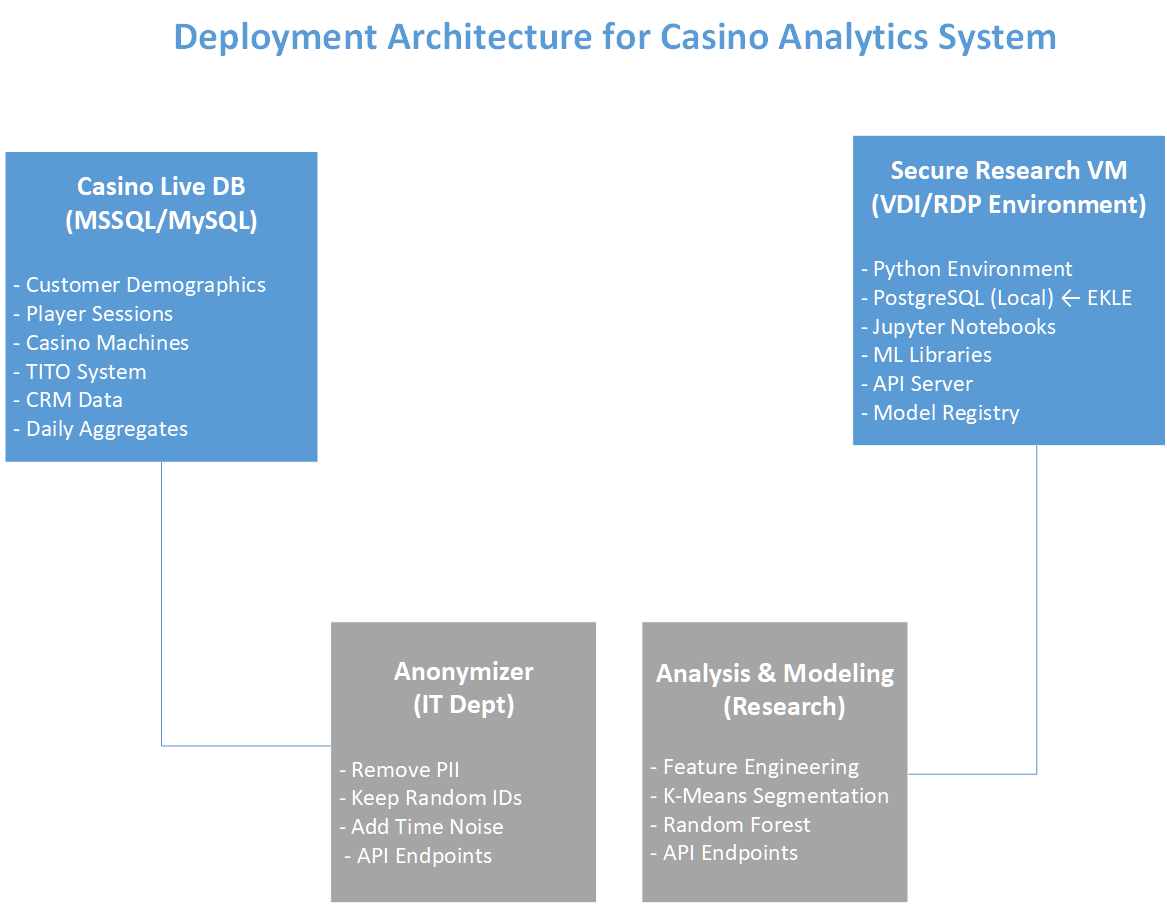
\includegraphics[width=0.85\textwidth]{figures/casino_analytics_system.png}
%\caption{Deployment Infrastructure for Casino Analytics System: DB, VM, and Security Layers}
\label{fig:deployment-architecture}
\end{figure}


Figure~\ref{fig:deployment-architecture} Illustrates the system’s deployment and anonymisation flow between live databases and the research environment.


\subsection{Data Context and Research Setting}

This research is carried out in the context of a physical casino in Eastern Europe, utilising anonymised player data gathered from slot machine activity, ticket-in ticket-out (TITO) logs, and historical customer relationship management (CRM) interactions.  The main data sources consist of two live relational databases—MSSQL and MySQL—integrated via secure anonymisation protocols and subsequently transferred to a PostgreSQL research environment. 

 This study utilises 12 months of behavioural logs from January to December 2022, encompassing more than 30,000 unique player records.  In the absence of comprehensive demographic data, synthetic demographic attributes, including age group, gender, and nationality, have been produced algorithmically as a synthetic data using Python's library. This approach ensures GDPR compliance while facilitating socio-demographic segmentation \citep{gdpr2016}.

 The data was accessed through remote desktop protocol (RDP) with supervision from the casino’s IT department, ensuring compliance with ethical guidelines approved under reference 10351-12382 by the University of Bath.  Personally identifiable information (PII) was excluded at the source, and all customer identifiers were either hashed or pseudonymized.

 The controlled environment guided the simulation of real-world marketing scenarios while following to data privacy regulations.  The research setting demonstrates a pragmatic design that emulates operational casino systems, providing a flexible and modular framework for academic experimentation.


\subsection{System Objective and Target Use Case}


\subsection{CRM Compatibility and Real-Time Utility}


%-------------------------------------------------------------------------------
\section{Contributions}

The goal of this study was to create AI-based solutions for high-frequency transactional settings, where customer behaviour can be tracked and dealt with in real time.  The gambling domain has a special mix of high transaction volume, a wide range of users, and marketing responsiveness.  Unlike more established AI fields like healthcare or e-commerce, retail, gaming, especially physical casinos, hasn't been studied much in university AI applications.  This project aims to fill that gap by mixing real data, ethical design principles, and an AI pipeline that can be used in any way.

As a researcher, "I deliberately selected a domain with high transaction volume but relatively low academic saturation in AI implementation, enabling more originality and freedom for system design."

The dissertation presents the following key contributions:

\begin{itemize}
    \item A hybrid data architecture that integrates slot machine logs and TITO records, producing CRM-compatible outputs, within a PostgreSQL database.
    \item A Python-based modular AI pipeline engineered for scalability and delivered via Docker, featuring custom feature engineering that encompasses behavioural volatility and loss-chasing detection.
    \item A segment-aware Random Forest model for promotional decision-making, underpinned by comparison analysis across client segments.
    \item A comparative model analysis and promotional decision-support logic.
\end{itemize}

\subsection*{1.4.1 Use of Generative AI Tools (Type B Declaration)}

Throughout the composition of this dissertation, the use of generative AI tools was restricted in accordance with the University of Bath's directives on Type B assessments. ChatGPT-4 (OpenAI, \url{https://chat.openai.com/}) was utilised to aid in the preliminary creation of some non-essential code segments and to validate Python syntax throughout the implementation stage.

The AI aid was restricted to the subsequent activities:
\begin{itemize}
    \item Validating and troubleshooting common Python constructs (e.g., pandas joins, stratified K-Fold validation)
    \item Analysing usage patterns of sklearn, such as parameters of RandomForestClassifier
    \item Proposing a framework for modular pipeline components, such as model evaluation functions
    \item Establishing preliminary formatting for visualisation code (matplotlib/seaborn)
\end{itemize}

All AI-generated content was examined, modified, and incorporated by the author, and no directly replicated code or text was utilised in the final dissertation. The conceptual design, technical rationale, implementation choices, and integration with the PostgreSQL/Docker pipeline were completely created and owned by the student. The utilisation of AI was not crucial for the project's completion and functioned only as an additional coding assistant.

%-------------------------------------------------------------------------------

%%%%%%%%%%%%%%%%%%%%%%%%%%%%%%%%%%%%%%%%%%%%%%%%%%%%%%%%%%%%%%%%%%%%%%%%%%%%%%%%
%%%%%%%%%%%%%%%%%%%%%%%%%%%%%%%%%%%%%%%%%%%%%%%%%%%%%%%%%%%%%%%%%%%%%%%%%%%%%%%%
\chapter{Literature and Technology Survey}

The convergence of artificial intelligence (AI), demographic analytics, and customer engagement represents a critical domain of innovation in the casino industry.  Although considerable research has investigated the implementation of machine learning in online gaming platforms, the use of AI-driven systems in physical casino settings is still restricted.  This chapter provides a critical examination of recent studies related to fundamental concepts, technologies, and models linked to AI-driven segmentation, prediction, and operational optimisation in casinos.   This review analyses clustering techniques, including K-Means, and evaluates supervised models such as Random Forest, while comparing various algorithms. It also explores the influence of demographics on player behaviour and discusses frameworks for responsible gambling. Additionally, technological frameworks like TITO systems, which offer readily available data for CRM integration, and real-time data pipelines are examined in the context of recent advancements.

\section{Artificial Intelligence in Casino Environments}
Recent advancements in artificial intelligence have enabled new forms of player engagement and dynamic personalisation in casino operations \citep{Auer2023, Omike2022a}. Studies show that predictive model Random Forest can increase player retention and optimise marketing strategies \citep{Ladouceur2016}.


\section{Demographic Segmentation and Behavioural Profiling}

Understanding the influence of demographic attributes on gambling activity is crucial for customer segmentation and targeted marketing strategies in physical casino environments.  Important demographic characteristics, including as age, gender, nationality, and socioeconomic status, have been shown to correlate with gaming preferences, betting habits, and overall engagement duration \citep{Hing2014}. For instance, younger players are typically linked to frequent, low-value gaming sessions, whereas older groups generally engage in longer play periods and make greater average wagers \citep{Desiata2024b}.

Segmenting casino customers based on demographic factors provides operational advantages such as personalised promotions, game-floor layout optimisation, and differentiated loyalty schemes. Studies have highlighted that tailored communication based on language or cultural preferences can increase return visits and ticket-in amounts \citep{Abarbanel2022}. Additionally, nationality-specific clustering has discovered behavioural differences; for example, visitors from the Balkan region demonstrate distinct slot preferences in contrast to those from Western Europe.

However, demographic segmentation in isolation may not be sufficient to predict customer lifetime value or risk profiles. Researchers advocate for combining demographic profiles with behavioural and transactional data to create multi-dimensional customer personas \citep{Ladouceur2016}. In line with this, our study integrates demographic attributes into behavioural clustering and prediction tasks, using them as input features for model training.

Data collected from physical casinos, particularly in multi-national tourist zones, presents unique opportunities for demographic profiling. Our dataset reflects such diversity, including anonymised player information across nationalities such as Bulgaria, Germany, Greece, Turkey, and the Netherlands. These insights are crucial for developing AI-powered recommendation systems that align with players' cultural expectations and risk tolerance.


\section{Clustering and Classification Algorithms}

Machine learning has enabled a wide range of data-driven strategies in casino analytics, particularly for customer segmentation and behavioural prediction. This study adopts a hybrid approach that leverages both unsupervised and supervised learning algorithms, tailored to the characteristics of anonymised player data collected from physical casino environments.

\subsection{K-Means Clustering}

K-Means is a widely used unsupervised algorithm for partitioning customers into behavioural segments.  The process involves minimising intra-cluster variance and allocating players to the nearest centroid within the feature space \citep{MacQueen1967}. K-Means clustering has been used in casino contexts to categorise players according to session duration, loss volatility, zone diversity, and average bet size.\citep{Desiata2024a}. The simplicity and interpretability of the algorithm make it especially suitable for initial segmentation in real-time applications.

This project utilised K-Means to categorise customers into three primary groups: Casual, Regular, and High Roller players.  The identified segments formed the foundation for informed promotional decision-making in later classification tasks.  The clustering analysis was carried out over several six-month intervals to assess customer migration patterns and temporal consistency.

\subsection{Random Forest Classifier}

Random Forest is a supervised ensemble learning technique that takes decision trees, recognised for its strength and ability to generalise effectively \citep{Breiman2001}. It generates several decision trees and consolidates their outcomes to produce final predictions, hence mitigating overfitting.  The model has demonstrated efficiency in managing behavioural datasets characterised by heterogeneous feature types and partly missing values \citep{Auer2023}.

The present study utilised Random Forest to forecast a player's probability to respond positively to promotional offers.  Features obtained from demographic and behavioural sources—including loss-chasing scores, recent activity levels, and section labels—were utilised in the training process.  Cross-validation results indicated that Random Forest surpassed baseline classifiers, including Logistic Regression and Decision Trees, over various intervals.

\subsection{Gradient Boosting as an Alternative}

While Gradient Boosting Machine Learning (GBML) was not applied in this work, it continues to be an impressive option to Random Forest.  GBML develops cumulative models progressively, enhancing weak learners to reduce prediction error \citep{Omike2022b}.Research comparing GBML and RF in gaming contexts suggests that GBML may provide higher precision in certain situations, although with heightened complexity and reduced clarity.

Due of the real-time objectives and interpretability requirements of physical casino systems, Random Forest was deemed the best suitable classifier.  Future endeavours may involve the application of GBML models to assess their effectiveness in high-precision targeting contexts.

\section{Responsible Gambling and Ethical AI}

The importance of ethical questions surrounding responsible gambling has grown in recent years, especially with the increasing integration of AI-driven systems into casino operations.  Regulations like the General Data Protection Regulation (GDPR) place severe constraints on the collection, processing, and use of personal and behavioural data \citep{gdpr2016}. In physical casinos, these concerns get worse by the real-time nature of player tracking and the risk of accidentally targeting vulnerable individuals.

The goal of engaging in responsible gambling is to reduce negative outcomes by recognising and addressing problematic gambling behaviours.  Several studies stress the significance of integrating behavioural risk indicators into AI decision-making pipelines. These signs can include long session durations, unexpected bet changes, or a tendency to chase losses \citep{Ladouceur2016, Priyadarshini2022}. These indications not only safeguard vulnerable players but also conform to the ethical obligations of operators.

This study employs a privacy-preserving methodology in accordance with GDPR and ethical research norms. All client data utilised in model training was entirely anonymised by the application of synthetic identities and manufactured demographic profiles developed using the Faker library \citep{faker2025}. Furthermore, segmentation and prediction results were evaluated against false-positive risks to prevent marketing offers to players displaying potential indicators of problem gambling.

Honesty and understanding are also aspects of ethical design.  The promotional decision system explored using rule-based overrides to guarantee human-in-the-loop evaluation in extreme instances.  According to Abarbanel and Phung (2022), designing gaming technology in a way that is both transparent and culturally sensitive helps to build trust among users and encourages long-term participation.

\section{Casino Technologies: TITO, CRM and Data Pipelines}

Transactional systems and customer records are used together in modern casinos to make sure that each player has a personalised experience and that staff can keep an eye on what players are doing.  Ticket-In Ticket-Out (TITO) systems were first made to replace coin-based payouts. Now they are a great way to collect information about how people behave.  Each ticket stores timestamps, machine interactions, and financial values. These can be put together to get session-level insights and trends of loss-chasing \citep{Nemis2024}.

Platforms for customer relationship management, or CRM, are another essential element, particularly when it comes to retaining valuable players.  Promotion history, contact preferences, and demographic information are frequently stored in these platforms.  However, in physical casinos, where several systems may function independently, integrating CRM data with real-time behavioural signals continues to be a challenge \citep{Wayne2024}.

The vital connection between these different sources and AI-powered decision engines is provided by data pipelines.  Scalable prediction systems must be able to ingest, process, and transform real-time game logs in high-frequency settings like casinos.  In order to facilitate prompt feature engineering and promotional decisions, technologies like PostgreSQL in conjunction with RESTful APIs or Kafka-style stream processors are being utilised more and more.  Although the potential of such structures has been shown in earlier research on online gambling, their use in traditional contexts is still in the early stages \citep{Omike2022a}.

The hybrid data architecture used in this study combines slot machine telemetry, CRM profiles, and TITO logs into a single AI pipeline.  While following to ethical and privacy norms, this infrastructure facilitates real-time segmentation and predictive modelling.

\section{Research Gap and Summary}

While significant progress has been made in applying AI to online gambling platforms, there is a noticeable gap in literature addressing the deployment of machine learning in physical casino environments. Most existing studies focus on digital contexts with controlled environments, where user data is consistently structured and readily available \citep{Auer2023, Omike2022a}. In contrast, real-world casino data is often fragmented, partially anonymised, and lacks standardisation, making model development and deployment considerably more challenging.

Furthermore, the integration of demographic data with behavioural indicators remains underexplored. Although some research has acknowledged the influence of age, gender, and nationality on gambling behaviour \citep{Hing2014, Desiata2024a}, few studies have systematically incorporated these features into real-time AI pipelines for segmentation and promotion. Similarly, while clustering algorithms such as K-Means and classifiers like Random Forest have been evaluated in isolation, comparative and integrated applications in operational casino environments are limited \citep{MacQueen1967, Breiman2001}.

The lack of responsible gambling mechanisms within AI-driven casino decision systems also presents an ethical void. Existing literature has called for more interpretable and fair systems \citep{Ladouceur2016, Abarbanel2022}, yet practical frameworks for combining ethical oversight with predictive analytics remain rare—particularly in non-digital venues.

This dissertation addresses these gaps by developing an end-to-end AI-powered customer engagement framework tailored for physical casinos. The system integrates demographic segmentation, behavioural feature engineering, and predictive modelling within a privacy-preserving, real-time data architecture. It contributes to the field by bridging theoretical AI models with real-world deployment constraints and ethical considerations in a regulated environment.


%%%%%%%%%%%%%%%%%%%%%%%%%%%%%%%%%%%%%%%%%%%%%%%%%%%%%%%%%%%%%%%%%%%%%%%%%%%%%%%%
%%%%%%%%%%%%%%%%%%%%%%%%%%%%%%%%%%%%%%%%%%%%%%%%%%%%%%%%%%%%%%%%%%%%%%%%%%%%%%%%
\section{Overview of System Goals and Constraints}

The goal of this project is to create and use an AI-powered decision support system that makes customers more interested in going to real-life casinos by dividing them into groups in real time and predicting who they will be interested in what promotions they will see.  By using flexible machine learning models, the main goal is to close the gap between the rich behavioural data that is collected on-site and marketing insights that can be put into action.

The system is engineered to process client data from many sources, including Ticket-In Ticket-Out (TITO) logs, client Relationship Management (CRM) profiles, and slot machine telemetry.  The diverse inputs are consolidated via a PostgreSQL-supported data pipeline and are utilised in both clustering (K-Means) and classification (Random Forest) models.

Key objectives of the system include:

\begin{itemize}
  \item Segmenting players into behavioural groups to enable targeted marketing strategies.
  \item Predicting promotional responsiveness to minimise marketing waste and improve ROI.
  \item Ensuring GDPR-compliant data handling through anonymisation and consent-aware logic.
  \item Supporting both batch and real-time workflows for flexibility in deployment.
  \item Providing explainable results that can be reviewed and adjusted by CRM managers.
\end{itemize}

However, several operational and ethical constraints must be acknowledged. Real-world casino environments are constrained by limited data access, system integration issues, and the need for real-time responsiveness. Moreover, ethical requirements such as fairness, transparency, and responsible gambling must be integrated into every decision-making layer. These constraints directly influence the architecture, feature selection, and model design choices adopted throughout this dissertation.

\section{Functional and Non-Functional Requirements}

The system requirements for the proposed AI-powered casino engagement framework are categorised into functional and non-functional requirements. These requirements were derived through iterative development, literature-informed design principles, and real-world casino data constraints.

\section{Functional and Non-Functional Requirements}

A two-phase implementation strategy is employed to define the requirements of the proposed AI-based casino engagement framework: an exploratory phase (Casino-1) that employs synthetic datasets, and a production-aligned phase (Casino-2) that employs anonymised bulk data from real operational sources.  Non-functional requirements define how the system should perform under a variety of constraints, such as ethical, legal, and performance aspects, while functional requirements specify what the system must do.

\subsection{Functional Requirements}

\begin{enumerate}[label=FR\arabic*:]
  \item \textbf{Customer Anonymisation:} The system shall anonymise all customer identifiers using GDPR-compliant formats (e.g., \texttt{CUST\_XXXXXX}).\hfill \textit{(High)}
  
  \item \textbf{Synthetic Demographics:} The system shall generate synthetic demographic attributes (age range, gender, nationality) when they are unavailable, thereby guaranteeing GDPR-compliant pseudonymization \hfill \textit{(High)}
  
  \item \textbf{Secure Storage:} Demographic data shall be stored in the PostgreSQL schema \texttt{casino\_data.customer\_demographics}.\hfill \textit{(High)}
  
  \item \textbf{Feature Engineering:} The system shall extract behavioural features (e.g., \texttt{avg\_bet}, \texttt{loss\_rate}, \texttt{session\_duration}, \texttt{zone\_diversity}) from gameplay logs.\hfill \textit{(High)}
  
  \item \textbf{Customer Segmentation:} All active customers shall be segmented into \textit{Casual}, \textit{Regular}, and \textit{High Roller} groups using the K-Means algorithm.\hfill \textit{(High)}
  
  \item \textbf{Promotion Prediction:} A Random Forest classifier shall predict whether a promotion should be sent to a customer based on behavioural and demographic features.\hfill \textit{(High)}
  
  \item \textbf{Versioned Output:} All model outputs shall be saved with metadata under \texttt{casino\_data.customer\_features} for traceability.\hfill \textit{(Medium)}
  
  \item \textbf{REST API:} A RESTful endpoint shall return a customer's segment and promotion status upon querying by customer ID.\hfill \textit{(Medium)}
  
  \item \textbf{Multi-Source Ingestion:} The system shall support data ingestion from batch (.csv) and live session logs (MSSQL, MySQL).\hfill \textit{(Medium)}
  
  \item \textbf{Decision Logging:} Each AI decision shall be logged with timestamp, customer ID, and associated prediction probability for auditability and A/B testing.\hfill \textit{(Medium)}
\end{enumerate}

\subsection{Non-Functional Requirements}

\begin{enumerate}[label=NFR\arabic*:]
  \item \textbf{GDPR Compliance:} All personal data must be anonymised and pseudonymised in accordance with Article 26 of GDPR.\hfill \textit{(High)}
  
  \item \textbf{Reproducibility:} All model training pipelines and outputs shall be version-controlled and reproducible under fixed seeds and documented configurations.\hfill \textit{(High)}
  
  \item \textbf{Batch Performance:} The system shall complete segmentation for 50,000 customers within 5 minutes in offline mode.\hfill \textit{(Medium)}
  
  \item \textbf{Real-Time Response:} Prediction API endpoints shall respond within 300 milliseconds under normal server conditions.\hfill \textit{(Medium)}
  
  \item \textbf{Secure Connections:} All external database connections (e.g., MSSQL) shall use encrypted channels (e.g., over VPN/RDP).\hfill \textit{(High)}
  
  \item \textbf{Explainability:} Each prediction shall be stored alongside feature importances and timestamp for audit and human-in-the-loop review.\hfill \textit{(High)}
  
  \item \textbf{Modularity:} The system shall be designed modularly to allow the integration of new features or model types without architectural rewrites.\hfill \textit{(Medium)}
  
  \item \textbf{Bias Prevention:} Synthetic data generation shall maintain demographic balance to prevent model bias across age, gender, and nationality groups.\hfill \textit{(High)}
  
  \item \textbf{Academic Compliance:} All code, data access, and documentation shall comply with University of Bath’s ethical research standards and academic integrity guidelines.\hfill \textit{(High)}
  
  \item \textbf{Data Confidentiality:} Sensitive data files shall be excluded from public repositories and stored securely in protected storage environments.\hfill \textit{(High)}
\end{enumerate}

\section{Data Requirements and Ethics Constraints}

The system depends on consumer and transactional data from real casino settings, derived from three main sources: Ticket-In Ticket-Out (TITO) logs, slot machine telemetry, and consumer Relationship Management (CRM) profiles.  The data types vary in structure and granularity, requiring schema-aware input and preprocessing mechanisms.

\subsection*{Data Sources and Structure}

To test its early algorithms, the system's prototype (Casino-1) employed XML, CSV, and JSON files containing synthetic data.  Alternatively, a PostgreSQL-based pipeline was utilised in the final implementation (Casino-2) to load pre-anonymized transactional logs produced from MSSQL and MySQL systems.  The most important ones were:

\begin{itemize}
  \item \textbf{Slot Logs:} Session-level gameplay data including \texttt{bet\_amount}, \texttt{win\_amount}, \texttt{RTP}, \texttt{symbol\_patterns}, \texttt{session\_duration}.
  \item \textbf{TITO Logs:} Ticket-based cash flow data covering \texttt{ticket\_in}, \texttt{ticket\_out}, and jackpot contributions.
  \item \textbf{CRM Data:} Demographic attributes such as age, gender, nationality, VIP status, registration month, and communication preferences.
\end{itemize}

With timestamps included in every log entry, trend and volatility calculations are made possible, which greatly helps in temporal analysis and customer lifecycle modelling.

\subsection*{Anonymisation and GDPR Compliance}

In compliance with Article 26 of the General Data Protection Regulation (GDPR), the system applies a pseudonymisation protocol where customer identifiers are replaced with randomised, irreversible tokens in the format \texttt{CUST\_XXXXXX}. This ensures that individual identities cannot be inferred, even when multiple data sources are cross-linked.

Additionally:

\begin{itemize}
  \item Raw age values are converted into categorical ranges (e.g., 18–24, 25–34) to prevent individual reidentification.
  \item No names, email addresses, phone numbers, or biometric data are used or processed at any stage.
  \item All CRM demographic data were either anonymised or synthetically generated using the \texttt{Faker} Python library \citep{faker2025}.
\end{itemize}

\subsection*{Ethics Approval and Data Scope}

This project was conducted under the University of Bath’s ethical research guidelines and received formal ethics approval (Ref: 10351-12382) \citep{bathEthics}. Only aggregated and anonymised data has been used and there is no commercial agreement or operational deployment between the researcher and the casino operator.  All data handling procedures were structured in accordance to privacy-by-design principles, thereby preventing continuous monitoring or individual profiling.

%%%%%%%%%%%%%%%%%%%%%%%%%%%%%%%%%%%%%%%%%%%%%%%%%%%%%%%%%%%%%%%%%%%%%%%%%%%%%%%%
%%%%%%%%%%%%%%%%%%%%%%%%%%%%%%%%%%%%%%%%%%%%%%%%%%%%%%%%%%%%%%%%%%%%%%%%%%%%%%%%
\chapter{Design}

\section{System Architecture and Module Overview}

The architecture of the Casino AI decision-support system is structured to manage real-world operational data, facilitate modular testing, provide explainable outputs, and ensure ethical data processing.  The system comprises four primary pipeline phases, each aligned with a separate phase in the analytical workflow..

\subsection{Modular Pipeline Phases}

\begin{itemize}

  \item \textbf{Phase 0 \textendash{} Data Ingestion and Schema Management:} 
  This step involves combining batch and real-time data from MSSQL and MySQL sources into a PostgreSQL-based research model. Distinct tables are preserved for raw logs, engineered features, promotional decisions, and audit tracking.

  \item \textbf{Phase 1 \textendash{} Feature Engineering Layer:} 
  This phase conducts behavioural and temporal analysis of slot gameplay and TITO transactions. Engineered measures encompass session volatility, loss-chasing indicators, zone variety, and recency measurements. These features are informed by prior work on behavioural clustering and predictive segmentation in gaming environments \citep{Desiata2024b, Omike2022b}. All attributes are organised in a structured table associated with each anonymised client ID.

  \item \textbf{Phase 2 \textendash{} AI Modelling and Inference:} 
  K-Means clustering is applied for behavioural segmentation (Casual, Regular, High Roller), followed by Random Forest classification to determine suitability for promotional offers. Every prediction is recorded with version control and metadata for the purpose of auditability.

  \item \textbf{Phase 3 \textendash{} CRM Integration and API Access:} 
  The prediction engine's results are accessible via a RESTful FastAPI endpoint, enabling CRM managers to query player segmentation and promotional decisions. An A/B testing framework is integrated into the output logging layer for offline assessment.

\end{itemize}

\subsection{System Components}

The system consists of the following interacting modules:

\begin{itemize}
  \item \textbf{Database Layer (PostgreSQL):} Stores all ingested data, features, model outputs, and metadata.
  \item \textbf{Data Preprocessing Scripts:} Written in Python, these transform raw logs into clean, model-ready features.
  \item \textbf{AI Models:} KMeans and Random Forest modules stored under \texttt{src/models/}, versioned and documented.
  \item \textbf{API Layer:} A FastAPI application exposes endpoints for real-time CRM queries.
  \item \textbf{Audit Layer:} Logs model runs, decisions, features used, and promotion outcomes in a separate schema for traceability.
\end{itemize}

\subsection{Feature Engineering}

As an important part of this project's analysis, feature engineering turns raw business logs into useful indicators of how players will act.  The system pulls out temporal and behavioural information from TITO transactions, slot machine sessions, and patterns of moving within the casino zone map.

The engineered features include:

\begin{itemize}

  \item \textbf{Session Duration Volatility:} Checks for unusual or repetitive play habits by measuring changes in session lengths. Session-level fluctuations are frequently analysed in behavioural tracking studies to detect compulsive patterns \citep{Abarbanel2022, Hing2014}.

  \item \textbf{Loss Chasing Score:} Based on total session trajectories, this number shows whether the player tends to raise bet amounts or session lengths after losing. This indicator corresponds to known psychological phenomena of chasing losses in gambling literature \citep{Ladouceur2016, Hing2014}.

  \item \textbf{Zone Diversity:} Shows how many different areas of place a player visits during busy gaming windows. This could mean that they are exploring or playing strategically. Zone-level activity variance has been used in prior work to characterise decision styles and targeted exploration in casino environments \citep{Omike2022c}.

  \item \textbf{Recency Index:} Keeps track of how recently the player has done something within a particular viewing window, like the last 7 or 30 days. Recency metrics are essential in churn modelling, retention scoring, and reactivation strategies \citep{Desiata2024b}.

  \item \textbf{Bet Trend Ratio:} Determines the pace of change in bet values over time, which can be used to detect signs of engagement or rising danger. Gradual shifts in betting behaviour have been associated with both high-value engagement and emerging risk \citep{Omike2022b, Hing2014}.

\end{itemize}

All features are stored under the \texttt{casino\_data.customer\_features} table in the PostgreSQL schema and linked via anonymised customer IDs. The features were selected with segmentation intends in consideration, and they have been supported by research on digital behavioural modelling \citep{Desiata2024b, Omike2022a, randomforest, kmeans}.

To preserve academic reproducibility and ensure compatibility with both batch and real-time pipelines, the feature calculations were implemented as modular functions in Python and executed on PostgreSQL-ingested datasets. This approach enables seamless export of feature sets for clustering and classification tasks downstream.

\subsection{Data Schema and Contextual Model}

The project uses a PostgreSQL-based relational database schema designed for casino analytics in order to support the modular pipeline architecture. Raw ingestion, feature computation, CRM feedback, and AI outputs are organised into logical domains within the schema, ensuring clean data separation. This structure promotes data integrity, GDPR compliance, and long-term auditability for academic and operational reproducibility.

\begin{itemize}

\item \texttt{casino\_data.customer\_demographics} \\
Contains anonymised customer IDs, grouped age ranges, gender, nationality, and registration month. All demographic data is synthetically generated under pseudonymisation and joint controllership.

\item \texttt{casino\_data.player\_sessions} \\
Stores individual slot machine session records, including session start/end times, total bet and win amounts, game type, and machine identifiers.

\item \texttt{casino\_data.tito\_transactions} \\
Tracks financial activity from Ticket-In-Ticket-Out (TITO) terminals. Each row links transaction IDs with customer and machine IDs, amount, and timestamps.

\item \texttt{casino\_data.customer\_features} \\
Holds engineered behavioural attributes (e.g., session duration volatility, loss chasing score, zone diversity) used for segmentation and prediction. All records are linked to anonymised customers and generation timestamps.

\item \texttt{casino\_data.customer\_temporal\_features} \\
Captures time-windowed indicators such as number of sessions in the last 30 days, volatility trends, and recent loss patterns. Used in temporal segmentation and Random Forest training.

\item \texttt{casino\_data.kmeans\_segments} \\
Stores segmentation outputs per customer per period (e.g., Casual, Regular, High Roller), including cluster IDs and model version references.

\item \texttt{casino\_data.kmeans\_segment\_metadata} \\
Maps k-means cluster numbers to interpretable labels and descriptions. Enables CRM-level understanding of segments across versions and time periods.

\item \texttt{casino\_data.temporal\_segments} \\
Tracks segment migration over rolling periods (e.g., from Casual to High Roller across two months). Enables retention and reactivation strategies.

\item \texttt{casino\_data.promo\_label} \\
Contains ground-truth labels (Low / Medium / High) used to train the promotional recommendation model. Generated based on behaviour-derived rules or CRM feedback.

\item \texttt{casino\_data.promotion\_history} \\
Simulated delivery and response data for promotional campaigns. Supports A/B testing and offline model evaluation.

\item \texttt{casino\_data.daily\_aggregates} \\
Summarised statistics of player activity per day: total sessions, total bet, total win/loss, average session duration.

\item \texttt{casino\_data.slot\_game\_catalog} \\
Static mapping of game types, categories (Slots, Poker, Blackjack), and metadata for analytical filtering.

\item \texttt{casino\_data.analysis\_periods} \\
Holds the defined monthly or quarterly windows used to align segmentation and feature generation processes.

\item \texttt{casino\_data.multi\_algorithm\_segments} \\
Stores outputs from non-KMeans models (e.g., DBSCAN, GMM, Hierarchical) for comparative academic clustering evaluation.

\item \texttt{casino\_data.optimized\_session\_plan} \\
Tracks model-recommended scheduling and segmentation output for daily CRM targeting.

\item \texttt{casino\_data.customer\_behavior\_profiles} \\
Higher-level customer personas constructed by aggregating segmentation and temporal data. Used for qualitative interpretation.

\item \texttt{casino\_data.customer\_game\_preferences} \\
Encodes player preferences across game categories and machines based on historical usage patterns.

\item \texttt{academic\_audit.*} \\
All model training logs, parameter settings, prediction timestamps, and audit trails are stored in a dedicated schema for traceability and reproducibility.

\end{itemize}

This schema supports both batch-mode ingestion and real-time prediction, providing the flexibility for replicating future CRM campaigns under reliable, research-only conditions.  The framework was formulated according to contextual models defined in previous decision-support literature for retail and gaming systems \citep{Ghaharian2022, Abarbanel2022}.

\begin{figure}[H]
\centering
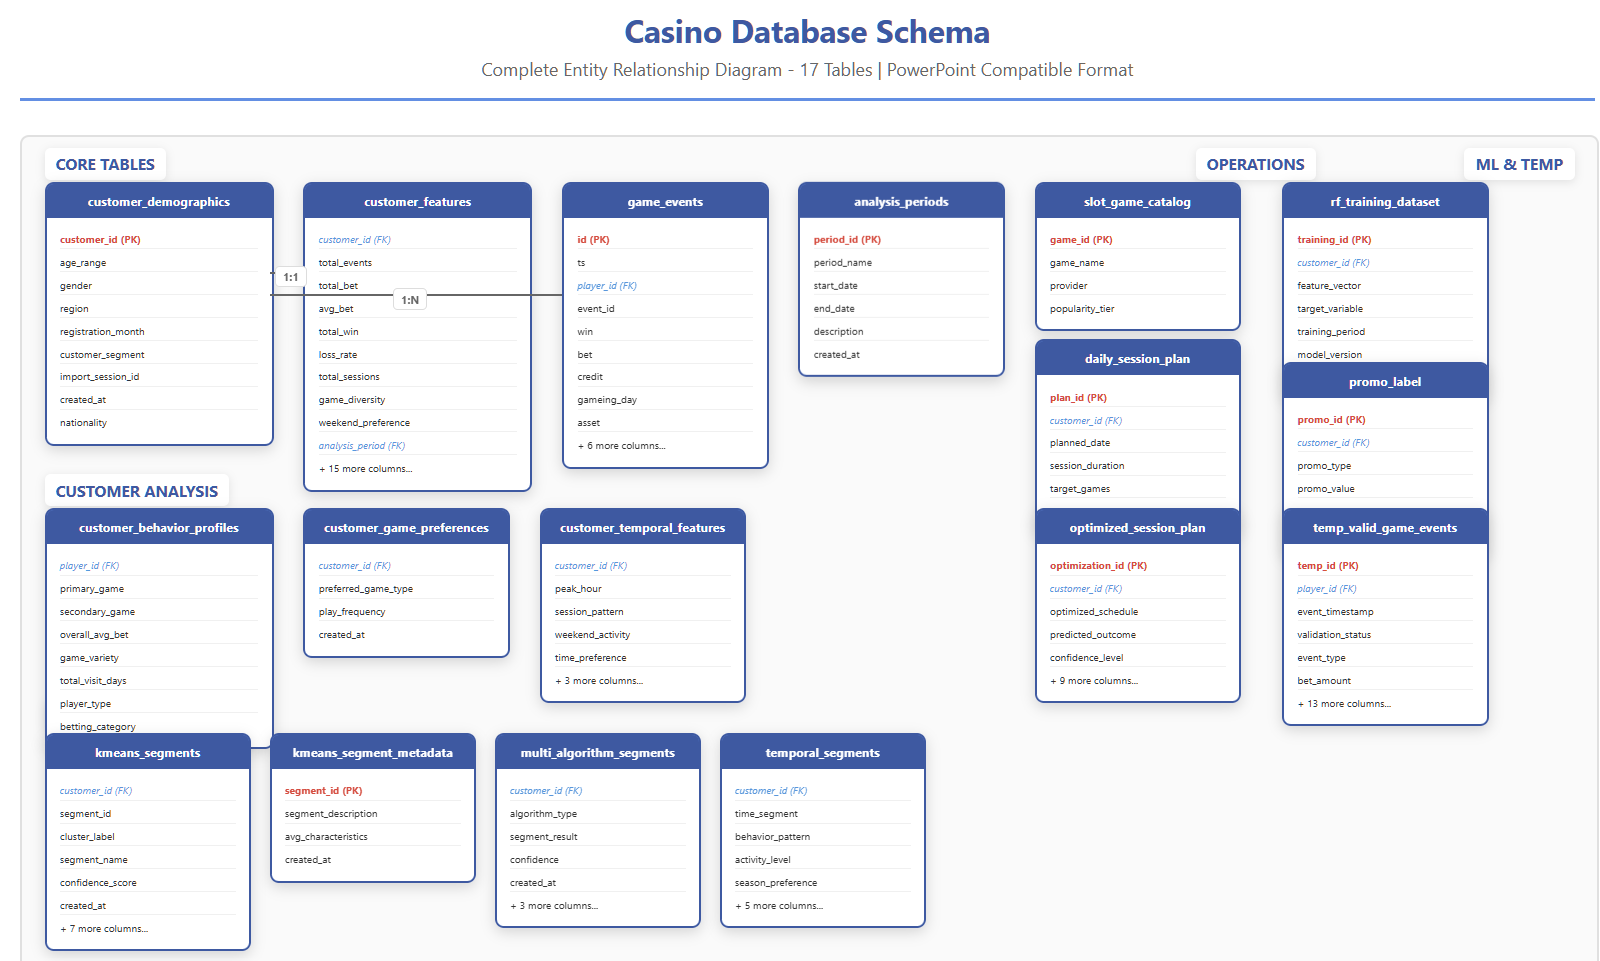
\includegraphics[width=\textwidth]{figures/casino_db_diagram.png}
\caption{PostgreSQL Schema Design for Casino-2 Analytical System}
\label{fig:casino_schema}
\end{figure}


\section{Data Flow and Component Interactions}

The main system is made to work with modular AI processes for dividing customers into groups and making decisions about promotions.  So, the internal data flow links preprocessing, feature extraction, model inference, and API contact parts in a way that can be repeated and is aware of audits.

\subsection{Pipeline Execution via \texttt{main\_pipeline.py}}

At the center of execution is \texttt{main\_pipeline.py}, a callable script that orchestrates the comprehensive data pipeline. It retrieves pre-defined analysis periods, fetches raw data from PostgreSQL, executes feature engineering functions, trains models as required, and stores predictions in the database.  The conditional logic of this module allows for the independent or batch activation of pipeline phases, such as KMeans or Random Forest, across many periods.

\subsection{Behavioural Segmentation with \texttt{segmentation.py}}

The \texttt{segmentation.py} module implements K-Means clustering based on engineered behavioural features. This includes:

\begin{itemize}
    \item Loading clean features from the database for a defined period
    \item Applying standardisation and cluster optimisation heuristics
    \item Mapping clusters into human-readable business labels (Casual, Roller, High Value players)
    \item Writing outputs to \texttt{casino\_data.kmeans\_segments} with versioning
\end{itemize}

It also contains rules and restrictions to exclude outliers or corrupted information (e.g., improper age or null sessions).  The ultimate cluster metadata is retained in \texttt{kmeans\_segment\_metadata} and periodically refreshed to support downstream analytics.

\subsection{Promotional Inference with \texttt{rf\_training.py}}

The \texttt{rf\_training.py} script serves as a supervised learning module for predicting promotional targeting based on segment-specific and behavioural features. Its structure includes:

\begin{itemize}
    \item Stratified sampling and GroupKFold cross-validation
    \item Optional hyperparameter tuning for reproducibility
    \item Integration of probabilistic labelling (e.g., Low, Medium, High impact)
    \item Saving trained models in Pickle format with logs in \texttt{academic\_audit}
\end{itemize}

The outputs of the Random Forest are evaluated using performance metrics and archived for subsequent A/B testing or CRM based simulations.

\subsection{CRM Interaction via RESTful API}

The prediction system is accessible through a FastAPI interface, if required, allowing CRM employees to retrieve segment labels and promotional recommendations for specific clients.  API endpoints are subject to rate limitations and are monitored for audit purposes.  All requests are processed through a logging layer that records timestamps, input parameters, and inference metadata according to the  \texttt{academic\_audit} schema.

\subsection{Component Map Overview}

\begin{itemize}
    \item \texttt{main\_pipeline.py} \textendash{} Central orchestrator for multi-period processing
    \item \texttt{feature\_engineering.py} \textendash{} Extracts features like volatility, recency, and loss chasing
    \item \texttt{segmentation.py} \textendash{} Applies KMeans clustering and stores segments with version control
    \item \texttt{rf\_training.py} \textendash{} Trains Random Forest model and logs artefacts
    \item \texttt{api.py} \textendash{} FastAPI interface for CRM-facing decision retrieval
    \item \texttt{db\_connector.py} \textendash{} Handles PostgreSQL interactions securely
\end{itemize}

This modular configuration ensures that any component can be evaluated, enhanced, or changed freely, allowing persistent scalability and scholarly reproducibility.

%-------------------------------------------------------------------------------

\subsection{AI Modelling and Inference}
\label{sec:ai_modelling_inference}

The modelling component of the Casino AI system is structured as a two-stage machine learning pipeline consisting of unsupervised segmentation and supervised promotional prediction. This pipeline was initially developed under a proof-of-concept prototype called \textbf{Casino-1}, using synthetically generated slot machine data and CRM profiles (approx. 1,500–2,000 records). In the production-aligned system \textbf{Casino-2}, the modelling logic was migrated to PostgreSQL-driven modules with anonymised real-world data and audit logging.

\subsubsection*{Behavioural Segmentation (K-Means)}

In Casino-1, segmentation was performed via the \texttt{train\_kmeans.py} module, which clusters customers into three behavioural groups based on engineered features including \texttt{avg\_loss}, \texttt{RTP}, \texttt{session\_duration}, and \texttt{zone\_diversity}, derived from preprocessed slot activity logs. Outputs were visualised in matplotlib-based diagrams (see Figure~\ref{fig:casino1_segmentation}) and stored as \texttt{labeled\_customer\_dataset.csv}. Segment labels were mapped into business-relevant profiles (e.g., Casual, Regular, High Roller).

\begin{figure}[H]
\centering
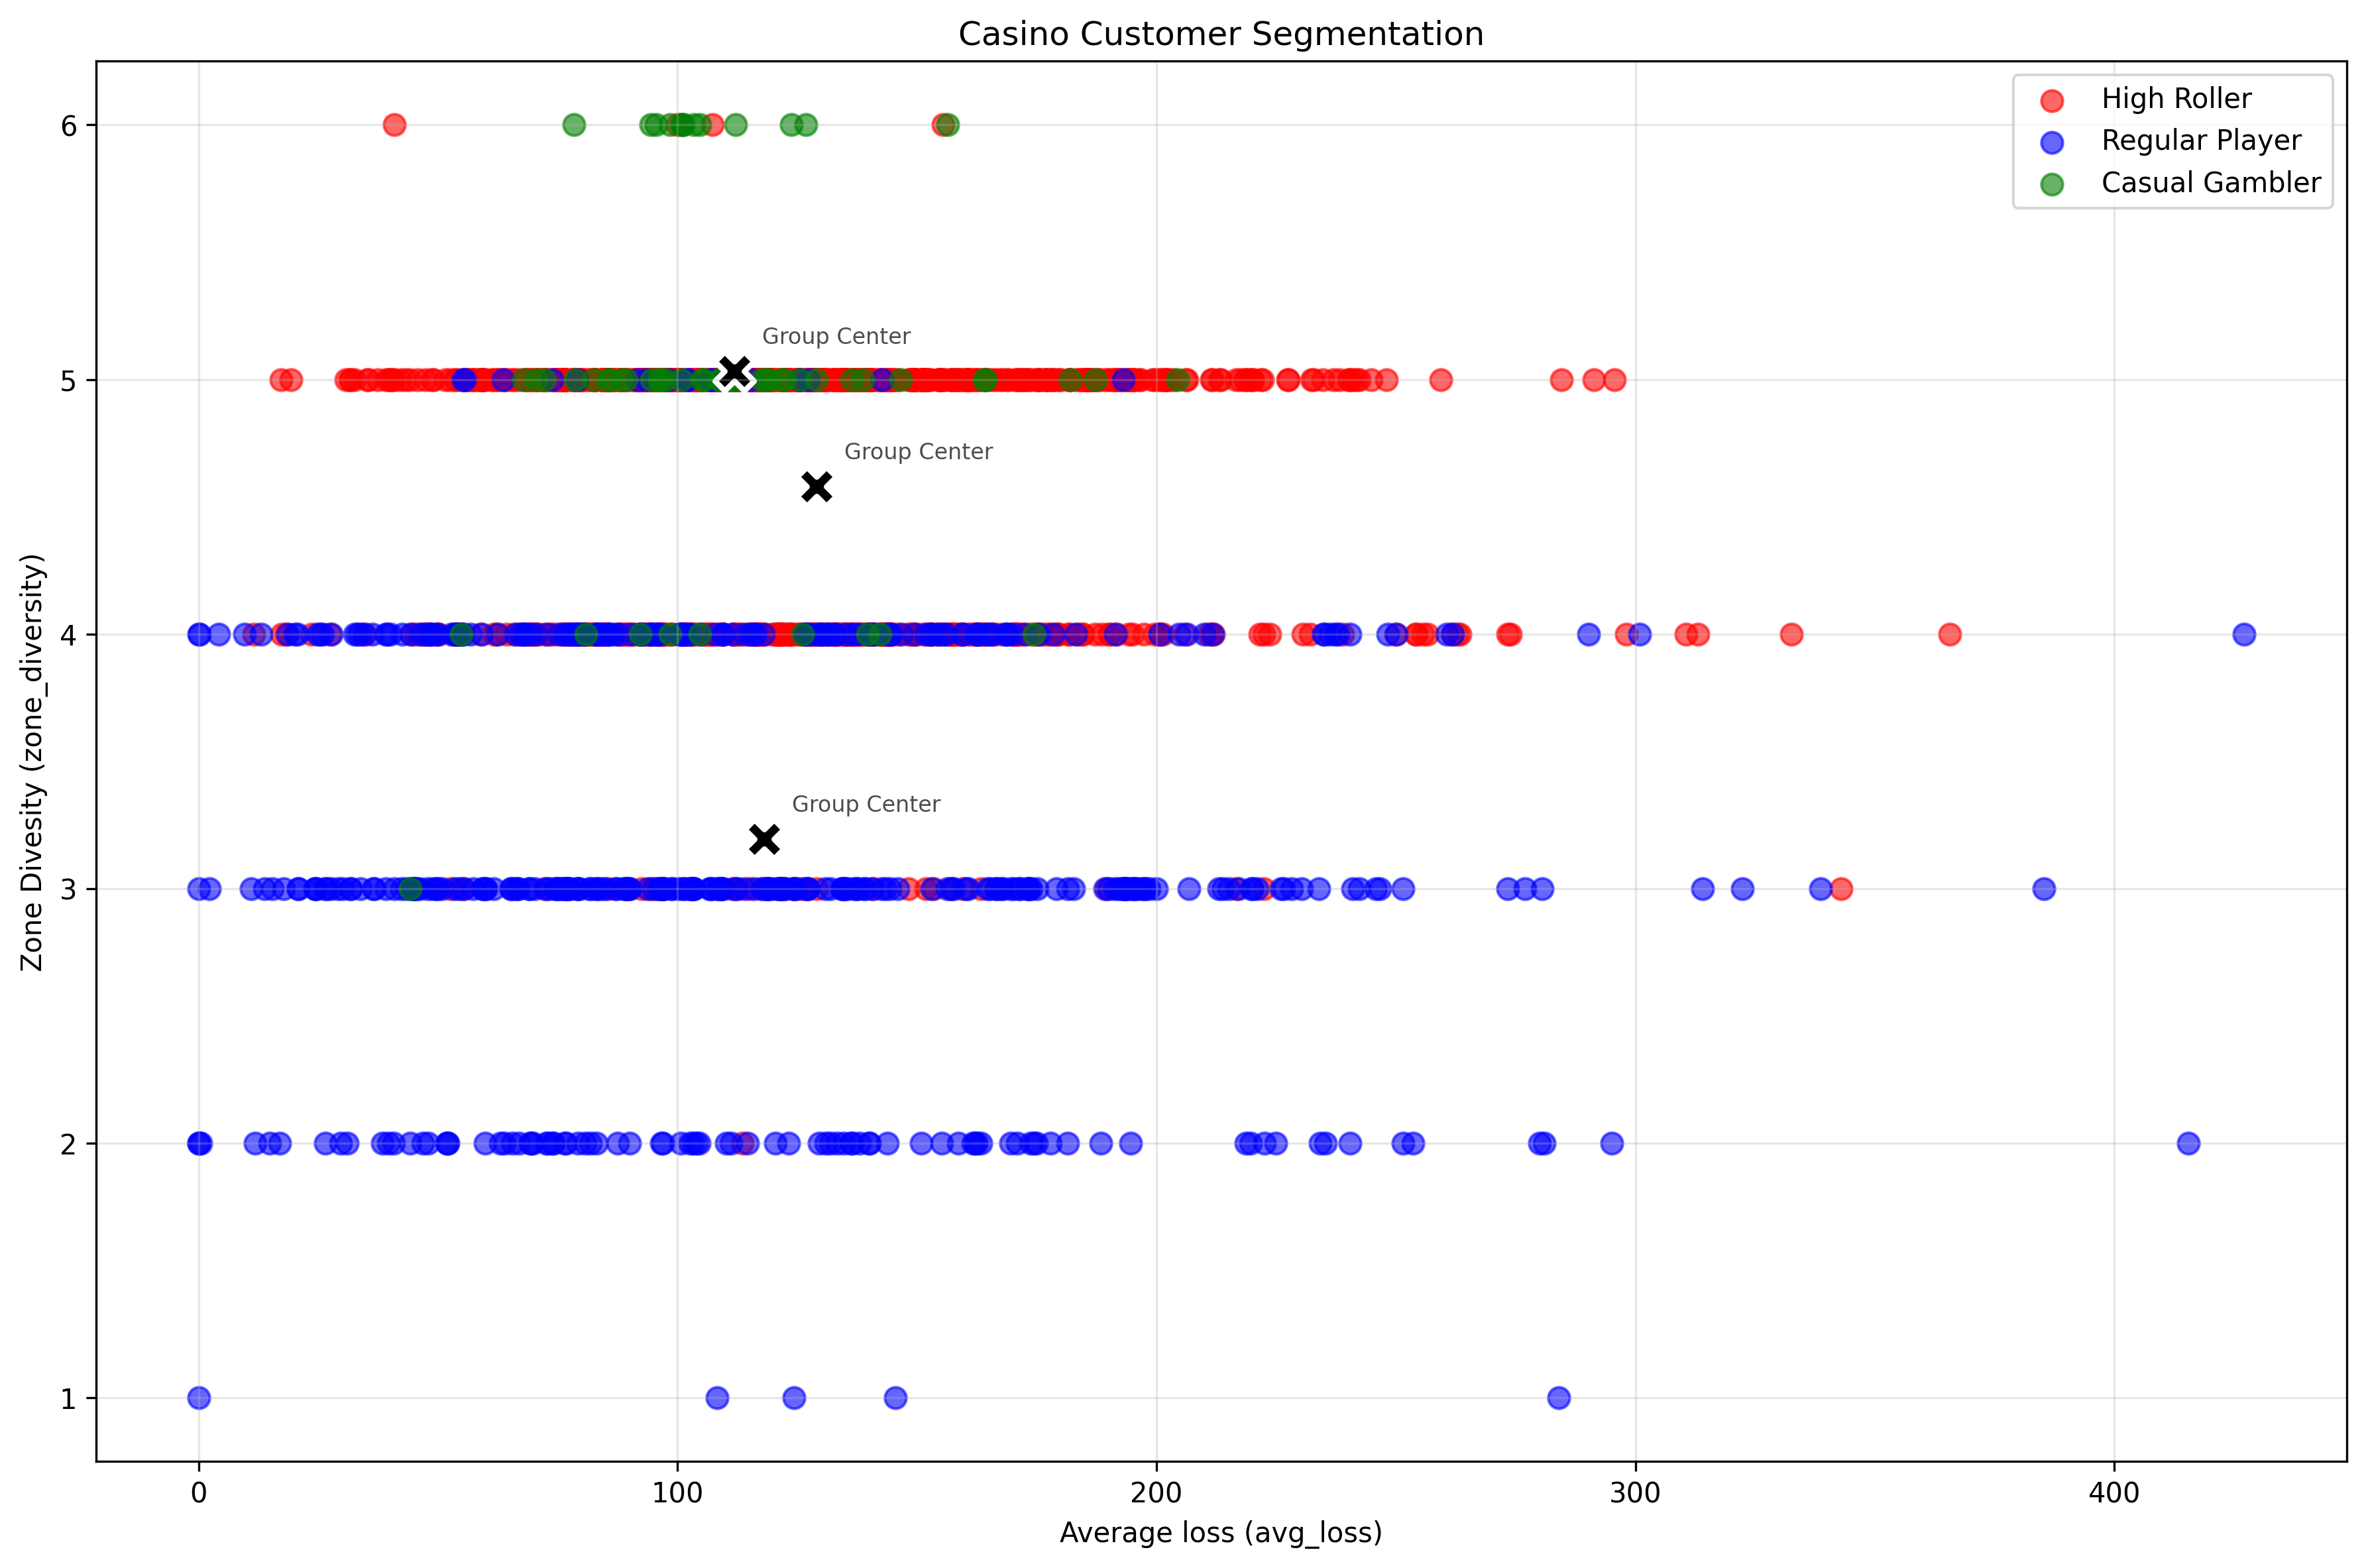
\includegraphics[width=0.8\textwidth]{figures/segmentation_analysis.png}
\caption{K-Means segmentation visualisation for Casino-1 dataset.}
\label{fig:casino1_segmentation}
\end{figure}

In Casino-2, the segmentation task was modularised and adapted to run on structured PostgreSQL tables. Multiple clustering algorithms including DBSCAN and Gaussian Mixture Models were also evaluated using the \texttt{multi\_algorithm\_segments} schema. Each segmentation task is linked to an \texttt{analysis\_period}, enabling longitudinal tracking (e.g., 2022-H1 to 2023-H2).

\subsubsection*{Promotional Prediction (Random Forest)}


Casino-2 transitioned this pipeline into fully auditable components, applying segment-based labelling and promotion flag harmonisation using domain-informed thresholds. Multiple modules such as \texttt{robust\_rf\_training\_major\_fix.py} and \texttt{enhanced\_rf\_promotion\_model.py} improved class balance, reproducibility, and cross-period generalisation.

Training was conducted independently on four half-year periods (2022-H1, 2022-H2, 2023-H1, 2023-H2) to detect seasonality and behavioural shifts. Feature importance scores and top predictive indicators (e.g., session volatility, bet trend ratio, zone diversity) were tracked across all model runs.

\subsubsection*{FastAPI Exposure and CRM Access}

In both environments, the prediction engine is served via REST endpoints. In Casino-1, this was implemented using \texttt{main.py} with local file inputs and matplotlib visual outputs for dashboard-style demonstration. In Casino-2, endpoints like \texttt{/segment} and \texttt{/promotion} were re-implemented with FastAPI, loading models from the registry and executing predictions on-demand using live features queried from the PostgreSQL database.

All model metadata, segment mappings, and feature logs are stored under the \texttt{academic\_audit} schema for reproducibility. A/B testing logs and future feedback loops are enabled by timestamped storage of prediction outcomes and CRM decisions.



%%%%%%%%%%%%%%%%%%%%%%%%%%%%%%%%%%%%%%%%%%%%%%%%%%%%%%%%%%%%%%%%%%%%%%%%%%%%%%%%
%%%%%%%%%%%%%%%%%%%%%%%%%%%%%%%%%%%%%%%%%%%%%%%%%%%%%%%%%%%%%%%%%%%%%%%%%%%%%%%%
\chapter{Implementation and Testing}

This is the chapter in which you review the implementation and testing decisions and issues, and critique these processes.

Code can be output inline using \verb@\lstinline|some code|@.  For example, this code is inline: \lstinline|public static int example = 0;| (we have used the character \verb@|@ as a delimiter, but any non-reserved character not in the code text can be used.)

Code snippets can be output using the \verb|\begin{lstlisting} ... \end{lstlisting}|
environment with the code given in the environment. For example, consider listing \ref{Example-Code}, below.

\begin{lstlisting}[breaklines,breakatwhitespace,caption={Example code},label=Example-Code]
public static void main() {

  System.out.println("Hello World");

}
\end{lstlisting}

Code listings are produced using the package `listings'.  This has many useful options, so have a look at the package documentation for further ideas.

%%%%%%%%%%%%%%%%%%%%%%%%%%%%%%%%%%%%%%%%%%%%%%%%%%%%%%%%%%%%%%%%%%%%%%%%%%%%%%%%
%%%%%%%%%%%%%%%%%%%%%%%%%%%%%%%%%%%%%%%%%%%%%%%%%%%%%%%%%%%%%%%%%%%%%%%%%%%%%%%%
\chapter{Results}

This is the chapter in which you review the outcomes, and critique the outcomes process. You may include user evaluation here too.


\subsection{Gradient Boosting Machine Learning (GBML)}

Gradient Boosting Machine Learning (GBML) has been extensively used in behavioural prediction tasks within casino analytics. In comparison to Random Forest, GBML offers enhanced predictive accuracy by sequentially addressing errors made by preceding learners. This advantage frequently entails longer training durations and diminished interpretability. While GBML was not utilised in this study, previous research indicates its effectiveness as an alternative for modelling promotional responses \citep{Omike2022b}. Future research could enhance understanding by comparing both models within real-time constraints and assessing segment-specific accuracy.


%%%%%%%%%%%%%%%%%%%%%%%%%%%%%%%%%%%%%%%%%%%%%%%%%%%%%%%%%%%%%%%%%%%%%%%%%%%%%%%%
%%%%%%%%%%%%%%%%%%%%%%%%%%%%%%%%%%%%%%%%%%%%%%%%%%%%%%%%%%%%%%%%%%%%%%%%%%%%%%%%
\chapter{Conclusions}

%%
%% Now we are back to the standard project contents that you should include
%%

This is the chapter in which you review the major achievements in the light of your original objectives, critique the process, critique your own learning and identify possible future work.

%%%%%%%%%%%%%%%%%%%%%%%%%%%%%%%%%%%%%%%%%%%%%%%%%%%%%%%%%%%%%%%%%%%%%%%%%%%%%%%%
%%%%%%%%%%%%%%%%%%%%%%%%%%%%%%%%%%%%%%%%%%%%%%%%%%%%%%%%%%%%%%%%%%%%%%%%%%%%%%%%


%%%%%%%%%%%%%%%%%%%%%%%%%%%%%%%%%%%%%%%%%%%%%%%%%%%%%%%%%%%%%%%%%%%%%%%%%%%%%%%%
%%%%%%%%%%%%%%%%%%%%%%%%%%%%%%%%%%%%%%%%%%%%%%%%%%%%%%%%%%%%%%%%%%%%%%%%%%%%%%%%
\appendix

%%
%% Use the appendix for major chunks of detailed work, such as these. Tailor
%% these to your own requirements
%%

%%%%%%%%%%%%%%%%%%%%%%%%%%%%%%%%%%%%%%%%%%%%%%%%%%%%%%%%%%%%%%%%%%%%%%%%%%%%%%%%
%%%%%%%%%%%%%%%%%%%%%%%%%%%%%%%%%%%%%%%%%%%%%%%%%%%%%%%%%%%%%%%%%%%%%%%%%%%%%%%%
\chapter{Design Diagrams}

%%%%%%%%%%%%%%%%%%%%%%%%%%%%%%%%%%%%%%%%%%%%%%%%%%%%%%%%%%%%%%%%%%%%%%%%%%%%%%%%
%%%%%%%%%%%%%%%%%%%%%%%%%%%%%%%%%%%%%%%%%%%%%%%%%%%%%%%%%%%%%%%%%%%%%%%%%%%%%%%%
\chapter{User Documentation}

%%%%%%%%%%%%%%%%%%%%%%%%%%%%%%%%%%%%%%%%%%%%%%%%%%%%%%%%%%%%%%%%%%%%%%%%%%%%%%%%
%%%%%%%%%%%%%%%%%%%%%%%%%%%%%%%%%%%%%%%%%%%%%%%%%%%%%%%%%%%%%%%%%%%%%%%%%%%%%%%%
\chapter{Raw Results Output}

%%%%%%%%%%%%%%%%%%%%%%%%%%%%%%%%%%%%%%%%%%%%%%%%%%%%%%%%%%%%%%%%%%%%%%%%%%%%%%%%
%%%%%%%%%%%%%%%%%%%%%%%%%%%%%%%%%%%%%%%%%%%%%%%%%%%%%%%%%%%%%%%%%%%%%%%%%%%%%%%%
\chapter{Code}

%% NOTE For this to typeset correctly, ensure you use the pdflatex
%%      command in preference to the latex command.  If you do not have
%%      the pdflatex command, you will need to remove the landscape and
%%      multicols tags and just make do with single column listing output

\begin{landscape}
\begin{multicols}{2}
\section{File: yourCodeFile.java}
\lstinputlisting[basicstyle=\scriptsize]{yourCodeFile.java}
\end{multicols}
\end{landscape}

\bibliographystyle{agsm}
\bibliography{references}

\end{document}
